\documentclass[11pt,table]{beamer}
\mode<presentation>
\usepackage{etex}
\usepackage{graphicx}
\usepackage{epstopdf}
\usepackage[english]{babel}
\usepackage{tabularx}
\usepackage{booktabs}
\usepackage{mathrsfs}
\usepackage{multicol}
\usepackage{bm}
\usepackage{subcaption}
\usepackage{wrapfig}
\usepackage{dcolumn}
\usepackage{threeparttable}
\usepackage{booktabs}
\usepackage{bbm}
\usepackage{amsmath,dsfont,listings}
\usepackage{amssymb}
\usepackage{rotating}
\usepackage{multirow}
\usepackage[authoryear]{natbib}
\usepackage{circledsteps}
\usepackage{tikz}
\usetikzlibrary{arrows,decorations.pathmorphing,backgrounds,fit,positioning,shapes.symbols,chains}
\setbeamertemplate{section in toc}[sections numbered]
\setbeamertemplate{caption}[numbered]

\bibliographystyle{Econometrica}

\setbeamersize{text margin right=3.5mm, text margin left=7.5mm}  % text margin
\setbeamersize{sidebar width left=0cm, sidebar width right=0mm}
\setbeamertemplate{sidebar right}{}
\setbeamertemplate{sidebar left}{}

\definecolor{text-grey}{rgb}{0.45, 0.45, 0.45} % grey text on white background
\definecolor{bg-grey}{rgb}{0.66, 0.65, 0.60} % grey background (for white text)
\definecolor{fu-blue}{RGB}{0, 51, 102} % blue text
\definecolor{fu-green}{RGB}{153, 204, 0} % green text
\definecolor{fu-red}{RGB}{204, 0, 0} % red text (used by \alert)

\setbeamertemplate{frametitle}{%
    \vskip-30pt \color{text-grey}\large%
    \begin{minipage}[b][23pt]{80.5mm}%
    \flushleft\insertframetitle%
    \end{minipage}%
}

\setbeamertemplate{navigation symbols}{} 

%%% begin title page
\setbeamertemplate{title page}{
\vskip2pt\hfill
\vskip6pt\hskip3pt

% set the title and the author
\vskip14pt
\parbox[top][1.35cm][c]{11cm}{\LARGE\color{text-grey}\inserttitle \\[1ex] \small \insertsubtitle \\[3ex]}
\vskip11pt
\parbox[top][1.35cm][c]{11cm}{\small \insertauthor \; \insertinstitute \\[2ex] \insertdate}
}
%%% end title page

%%% colors
\usecolortheme{lily}
\setbeamercolor*{normal text}{fg=black,bg=white}
\setbeamercolor*{alerted text}{fg=fu-red}
\setbeamercolor*{example text}{fg=fu-green}
\setbeamercolor*{structure}{fg=fu-blue}

\setbeamercolor*{block title}{fg=white,bg=black!50}
\setbeamercolor*{block title alerted}{fg=white,bg=black!50}
\setbeamercolor*{block title example}{fg=white,bg=black!50}

\setbeamercolor*{block body}{bg=black!10}
\setbeamercolor*{block body alerted}{bg=black!10}
\setbeamercolor*{block body example}{bg=black!10}

\setbeamercolor{bibliography entry author}{fg=fu-blue}
\setbeamercolor{bibliography entry journal}{fg=text-grey}
\setbeamercolor{item}{fg=fu-blue}
\setbeamercolor{navigation symbols}{fg=text-grey,bg=bg-grey}
%%% end colors

%%% headline
\setbeamertemplate{headline}{
\vskip30pt
}
%%% end headline

%%% footline
\newcommand{\footlinetext}{
%\insertshortinstitute, \insertshorttitle, \insertshortdate
}
\setbeamertemplate{footline}{
\vskip2pt
\hfill \raisebox{-1pt}{\usebeamertemplate***{navigation symbols}}
\hfill \insertframenumber\hspace{10pt}
\vskip4pt
}
%%% end footline

%%% settings for listings package
\lstset{extendedchars=true, showstringspaces=false, basicstyle=\footnotesize\sffamily, tabsize=2, breaklines=true, breakindent=10pt, frame=l, columns=fullflexible}
\lstset{language=Java} % this sets the syntax highlighting
\lstset{mathescape=true} % this switches on $...$ substitution in code
% enables UTF-8 in source code:
\lstset{literate={�}{{\"a}}1 {�}{{\"o}}1 {�}{{\"u}}1 {�}{{\"A}}1 {�}{{\"O}}1 {�}{{\"U}}1 {�}{\ss}1}
%%% end listings

\usepackage{concmath}
\usepackage{xcolor}
\definecolor{lightblue}{rgb}{0.8,0.85,1}
\definecolor{persianred}{rgb}{0.8, 0.2, 0.2}
\definecolor{red1}{RGB}{206, 17, 38}
\definecolor{blue1}{RGB}{16, 118, 208}
\definecolor{gray1}{RGB}{117, 115, 115}
\usepackage{hyperref}
\hypersetup{
    bookmarks=false,
    unicode=false,
    pdftoolbar=false,
    pdffitwindow=true,
    pdftitle={Econometricks: Short guides to econometrics},
    pdfauthor={Davud Rostam-Afschar},
    pdfsubject={econometrics},
    pdfcreator={Davud Rostam-Afschar},
    pdfproducer={Davud Rostam-Afschar},
    pdfkeywords={econometrics},
    pdfnewwindow=true,
}

\newtheorem{proposition}{Proposition}
\newtheorem{assumption}{Definition}

\title[] 
{Econome\textcolor{red1}{tricks}: Short guides to econometrics\\[1ex]\normalsize 
}

\author[D. Rostam-Afschar]{Trick 05:  Simplifying Linear Regressions using Frisch-Waugh-Lowell\\[2ex]}

\institute[]{\textcolor{gray1}{Davud Rostam-Afschar (Uni Mannheim)}}
            
\date[] 
{}

\subject{Econometrics}
\renewcommand{\footlinetext}{\insertshortinstitute, \insertshorttitle, \insertshortdate}

\def\sym#1{\ifmmode^{#1}\else\(^{#1}\)\fi}

\begin{document}

\begin{frame}[plain]
  \titlepage
\end{frame}

% --------------------------------------------------- Slide --
\begin{frame}
	\frametitle{Content}
	\tableofcontents[]
\end{frame}

												

\section{Frisch-Waugh-Lovell theorem in equation algebra}



\begin{frame}{\small From the multivariate to the bivariate regression}
Regress $y_i$ on two explanatory variables, where $x^{2}_i$ is the variable of interest and $x^{\text{1}}_i$ (or further variables) are not of interest.

\begin{eqnarray}
y_i =\beta_0+\beta_{2}x^{2}_i+\beta_{1}x^{\text{1}}_i+\varepsilon_i.\nonumber
\end{eqnarray}

Surprising and useful result:
\begin{itemize}
	\item We can obtain \textbf{exactly the same} coefficients and residuals from a regression two \textcolor{red1}{demeaned} variables
$$\tilde{y}_i=\beta_0+\beta_2\tilde{x}^{2}_i+\varepsilon_i.$$
	\item We can obtain \textbf{exactly the same} coefficient and residuals from a regression of two \textcolor{red1}{residualized} variables
	$$\varepsilon^{y}_i=\beta_{2}\varepsilon^{2}_i+\varepsilon_i.$$
\end{itemize}
\end{frame}


\begin{frame}{Why is the decomposition useful?}
Allows breaking a multivariate model with $K$ independent variables into $K$ bivariate models.
\small
\begin{itemize}
	\item Relationship between two variables from a multivariate model can be shown in a two-dimensional scatter plot
	\item Absorbs fixed effects to reduce computation time (see reghdfe for Stata)
	\item Allows to separate variability between the regressors (multicollinearity) and between the residualized variable $\tilde{x}^{2}_i$ and the dependent variable $y_i$.
	\item Understand biases in multivariate models tractably.
\end{itemize}
\end{frame}


\begin{frame}{How to decompose $y_i$ and $x^{2}_i$?}
Partial out $x^{1}_i$ from $y_i$ and from $x^{2}_i$.
\begin{itemize}
	\item Regress $x^{2}_i$ on all $x^{1}_i$ and get residuals $\varepsilon^{2}_i$:
	$$x^{2}_i=\gamma_0+\gamma_1x^{1}_i+\varepsilon^{2}_i,$$
	this implies $Cov(x^{1}_i,\varepsilon^{2}_i)=0,$
	\item Regress $y_i$ on all $x^{1}_i$ and get residuals $\varepsilon^{y}_i$:
	$$y_i=\delta_0+\delta_1x^{1}_i+\varepsilon^{y}_i.$$
	This implies $Cov(x^{1}_i,\varepsilon^{y}_i)=0.$
\end{itemize}
From the residuals and the constants $\gamma_0$ and $\delta_0$ generate
\begin{itemize}
	\item $\tilde{x}^{2}_i=\gamma_0+\varepsilon^{2}_i,$
	\item $\tilde{y}_i=\delta_0+\varepsilon^{y}_i.$
\end{itemize}
Finally,
$$\tilde{y}_i=\tilde{\beta}_0+\tilde{\beta}_1\tilde{x}^{2}_i+\tilde{\varepsilon}_i=\beta_0+\beta_2\tilde{x}^{2}_i+\varepsilon_i.$$	
\end{frame}

\begin{frame}{Decomposition theorem}
\begin{theorem}
\textbf{Decomposition theorem.} For multivariate regressions and detrended regressions, e.g.,
$$y_i =\beta_0+\beta_{2}x^{2}_i+\beta_{1}x^{1}_i+\varepsilon_i,$$
$$\tilde{y}_i=\tilde{\beta}_0+\tilde{\beta}_1\tilde{x}^{2}_i+\tilde{\varepsilon}_i,$$	
the same regression coefficients will be obtained with any non-empty subset of the explanatory variables, such that
$$\tilde{\beta}_1=\beta_2 \; \text{ and also }\; \tilde{\varepsilon}_i=\varepsilon_i.$$
\end{theorem}
\small Examining either set of residuals will convey precisely the same information about the properties of the unobservable stochastic disturbances.

\end{frame}

\begin{frame}{Detrended variables}
\small
Show that 
\begin{eqnarray}
y_i &=\beta_0+\beta_{2}x^{2}_i+\beta_{1}x^{1}_i+\varepsilon_i \label{orig}\\
&=\tilde{y}_i=\tilde{\beta}_0+\tilde{\beta}_1\tilde{x}^{2}_i+\tilde{\varepsilon}_i.
\end{eqnarray}
Plug in the variables $y_i=\delta_0+\delta_1x^{1}_i+\varepsilon^{y}_i$ and $x^{2}_i=\gamma_0+\gamma_1x^{1}_i+\varepsilon^{2}_i$ in the equation~\eqref{orig}
\begin{eqnarray}
y_i &=&\delta_0+\delta_1x^{1}_i+\varepsilon^{y}_i=\beta_0+\beta_{2}(\gamma_0+\gamma_1x^{1}_i+\varepsilon^{2}_i)+\beta_{1}x^{1}_i+\varepsilon_i\nonumber\\
\tilde{y}_i&=&\delta_0+\varepsilon^{y}_i=\beta_0+\beta_{2}(\gamma_0+\varepsilon^{2}_i)+(\beta_{2}\gamma_1-\delta_1+\beta_{1})x^{1}_i+\varepsilon_i.\nonumber
\end{eqnarray}
Because we partialled out $x^{1}_i$ using OLS, $x^{1}_i$ is mechanically uncorrelated to $\varepsilon^{2}_i$ and to $\varepsilon^{y}_i$. Therefore, the regression coefficient $(\beta_{2}\gamma_1-\delta_1+\beta_{1})$ of the partialled out variable $x^{1}_i$ is zero.
The equation simplifies with $\tilde{x}^{2}_i=\gamma_0+\varepsilon^{2}_i$ to
\begin{eqnarray}
\tilde{y}_i &=&\delta_0+\varepsilon^{y}_i=\beta_0+\beta_{2}(\gamma_0+\varepsilon^{2}_i)+\varepsilon_i.\nonumber
\end{eqnarray}

\end{frame}

\begin{frame}{Detrended variables}
\small
Regression anatomy: Only detrending $x^{2}_i$ and not $y_i$. The regression constant, residuals, and the standard errors change but $\beta_{2}$ remains
\begin{eqnarray}
y_i =\delta_0+\delta_1x^{1}_i+\varepsilon^{y}_i&=&(\beta_0+\delta_1\bar{x}^{1})+\beta_{2}(\gamma_0+\varepsilon^{2}_i)+(\varepsilon_i+\delta_1 x^{1}_i)\nonumber\\
y_i &=&\kappa+\beta_{2}\tilde{x}^{2}+\epsilon_i.
\end{eqnarray}
\end{frame}


\begin{frame}{Residualized variables}
\small
\begin{eqnarray}
\tilde{y}_i =\delta_0+\varepsilon^{y}_i&=&\beta_0+\beta_{2}(\gamma_0+\varepsilon^{2}_i)+\varepsilon_i\nonumber\\
\varepsilon^{y}_i&=&\beta_0-\delta_0+\beta_{2}\gamma_0+\beta_{2}\varepsilon^{2}_i+\varepsilon_i.\nonumber
\end{eqnarray}

The same result of the FWL Theorem holds as well for a regression of the residualized variables because $\beta_1=\delta_0-\beta_{2}\gamma_0$:
$$\varepsilon^{y}_i=\beta_{2}\varepsilon^{2}_i+\varepsilon_i.$$


\end{frame}


\section{Projection and residual maker matrices}



\begin{frame}{Partition of $\bm{y}$}
Least squares partitions the vector $\bm{y}$ into two orthogonal parts

$$\bm{y}=\bm{\hat{y}}+\bm{e}=\bm{Xb}+\bm{e}=\bm{Py}+\bm{My}.$$
\begin{itemize}
	\item $n \times 1$ vector of data $\bm{y}$
	\item $n \times n$ projection matrix $\bm{P}$
	\item $n \times n$ residual maker matrix $\bm{M}$
	\item $n \times 1$ vector of residuals $\bm{e}$
\end{itemize}
\end{frame}


\begin{frame}{Projection matrix}
\begin{eqnarray}
\bm{Py}&=&\bm{Xb}=\bm{X(X'X)^{-1}X'y}\nonumber\\
&&\nonumber\\
&&\rightarrow \bm{P}=\bm{X(X'X)^{-1}X'}.\nonumber
\end{eqnarray}

\begin{assumption} \textbf{Properties}. 
\begin{itemize}
	\item symmetric such that $\bm{P}=\bm{P}'$, thus orthogonal
	\item idempotent such that $\bm{P}=\bm{P}^2$, thus indeed a projection
	\item annihilator matrix $\bm{P}\bm{X}=\bm{X}$
\end{itemize}
\end{assumption} 
\end{frame}


\begin{frame}{Example for projection matrix}
\footnotesize
\begin{example}
Show $\bm{P}\bm{X}=\bm{X(X'X)^{-1}X'}\bm{X}=\bm{X}.$
\begin{eqnarray}
&&\textbf{X}=\begin{bmatrix}
1 & 0\\
1 & 1 \\
1 & 0
\end{bmatrix};
\textbf{X'X}=\begin{bmatrix}
1 & 1 & 1\\
0 & 1 & 0\\
\end{bmatrix}\begin{bmatrix}
1 & 0\\
1 & 1 \\
1 & 0
\end{bmatrix}=\begin{bmatrix}
3 & 1 \\
1 & 1 
\end{bmatrix};
\textbf{X'X}^{-1}=\begin{bmatrix}
1/2 & -1/2\\
-1/2 & 1.5 
\end{bmatrix};
\nonumber\\
&&\bm{X(X'X)^{-1}X'}=\begin{bmatrix}
1 & 0\\
1 & 1 \\
1 & 0
\end{bmatrix}
\begin{bmatrix}
1/2 & -1/2\\
-1/2 & 3/2 
\end{bmatrix}
\begin{bmatrix}
1 & 1 & 1\\
0 & 1 & 0\\
\end{bmatrix}=
\begin{bmatrix}
1/2 & 0 & 1/2\\
0 & 1 & 0\\
1/2 & 0 & 1/2
\end{bmatrix}
\nonumber\\
&&\bm{P}\bm{X}=\begin{bmatrix}
1/2 & 0 & 1/2\\
0 & 1 & 0\\
1/2 & 0 & 1/2
\end{bmatrix}\begin{bmatrix}
1 & 0\\
1 & 1 \\
1 & 0
\end{bmatrix}=\begin{bmatrix}
1 & 0\\
1 & 1 \\
1 & 0
\end{bmatrix}.
\end{eqnarray}
Project $\bm{y}$ on the column space of $\bm{X}$, i.e. regress $\bm{y}$ on $\bm{x}$ and predict $E[\bm{y}]=\bm{\hat{y}}.$
\begin{eqnarray}
\bm{y}=\begin{bmatrix}
1\\
2 \\
3
\end{bmatrix};
\bm{P}\bm{y}=\begin{bmatrix}
1/2 & 0 & 1/2\\
0 & 1 & 0\\
1/2 & 0 & 1/2
\end{bmatrix}\begin{bmatrix}
1\\
2 \\
3
\end{bmatrix}=\bm{\hat{y}}=\begin{bmatrix}
2\\
2 \\
2
\end{bmatrix}.
\end{eqnarray}
\end{example}


\end{frame}



\begin{frame}{Residual maker matrix}
\begin{eqnarray}
\bm{My}&=&\bm{e}=\bm{y}-\bm{Xb}=\bm{y}-\bm{X(X'X)^{-1}X'y}\nonumber\\
\bm{My}&=&(\bm{I}-\bm{X(X'X)^{-1}X')y}\nonumber\\
&&\nonumber\\
&&\rightarrow \bm{M}=\bm{I}-\bm{X(X'X)^{-1}X'}=(\bm{I}-\bm{P}).\nonumber
\end{eqnarray}

\begin{assumption} \textbf{Properties}. 
\begin{itemize}
	\item symmetric such that $\bm{M}=\bm{M}'$
	\item idempotent such that $\bm{M}=\bm{M}^2$
	\item annihilator matrix $\bm{M}\bm{X}=0$
	\item orthogonal to $\bm{P}$: $\bm{P}\bm{M}=\bm{M}\bm{P}=\bm{0}.$

\end{itemize}
\end{assumption} 


\end{frame}



\begin{frame}{Example for residual maker matrix}
\footnotesize
\begin{example}
Show $\bm{M}\bm{X}=(\bm{I}-\bm{X(X'X)^{-1}X'})\bm{X}=(\bm{I}-\bm{P})\bm{X}=\bm{X}-\bm{X}=\bm{0}.$
\begin{eqnarray}
&&\textbf{I}=\begin{bmatrix}
1 & 0 & 0\\
0 & 1 & 0\\
0 & 0 & 1 
\end{bmatrix};
\textbf{X}=\begin{bmatrix}
1 & 0\\
1 & 1 \\
1 & 0
\end{bmatrix};
\nonumber\\
&&\bm{M}=(\bm{I}-\bm{P})=\begin{bmatrix}
1 & 0 & 0\\
0 & 1 & 0\\
0 & 0 & 1 
\end{bmatrix}-\begin{bmatrix}
1/2 & 0 & 1/2\\
0 & 1 & 0\\
1/2 & 0 & 1/2
\end{bmatrix}=
\begin{bmatrix}
1/2 & 0 & -1/2\\
0 & 0 & 0\\
-1/2 & 0 & 1/2
\end{bmatrix}\nonumber\\
&&\bm{M}\bm{X}=\begin{bmatrix}
1/2 & 0 & -1/2\\
0 & 0 & 0\\
-1/2 & 0 & 1/2
\end{bmatrix}
\begin{bmatrix}
1 & 0\\
1 & 1 \\
1 & 0
\end{bmatrix}=\begin{bmatrix}
0 & 0\\
0 & 0 \\
0 & 0
\end{bmatrix}.
\end{eqnarray}
Obtain residuals from a projection of $\bm{y}$ on the column space of $\bm{X}$, i.e. regress $\bm{y}$ on $\bm{x}$ and predict $\bm{y}-E[\bm{y}]=\bm{y}-\bm{\hat{y}}.$
\begin{eqnarray}
\bm{y}=\begin{bmatrix}
1\\
2 \\
3
\end{bmatrix};
\bm{M}\bm{y}=\begin{bmatrix}
1/2 & 0 & -1/2\\
0 & 0 & 0\\
-1/2 & 0 & 1/2
\end{bmatrix}\begin{bmatrix}
1\\
2 \\
3
\end{bmatrix}=\bm{y}-\bm{\hat{y}}=\begin{bmatrix}
-1\\
0 \\
1
\end{bmatrix}.
\end{eqnarray}
\end{example}


\end{frame}




\begin{frame}{Example for residual maker matrix}
\footnotesize
\begin{example}
Column space of \textbf{X} is $\textbf{x}_0$ and $\textbf{x}_1$.
\begin{eqnarray}
\begin{bmatrix}
x^1_{0}=1 & x^1_{1}=0 & y^1=1\\
x^2_{0}=1 & x^2_{1}=1 & y^2=2\\
x^3_{0}=1 & x^3_{1}=0 & y^1=3 
\end{bmatrix};
\bm{\hat{y}}=\begin{bmatrix}
2\\
2 \\
2
\end{bmatrix};
\bm{y}-\bm{\hat{y}}=\begin{bmatrix}
-1\\
0 \\
1
\end{bmatrix}.
\end{eqnarray}
\begin{figure}
	\centering
		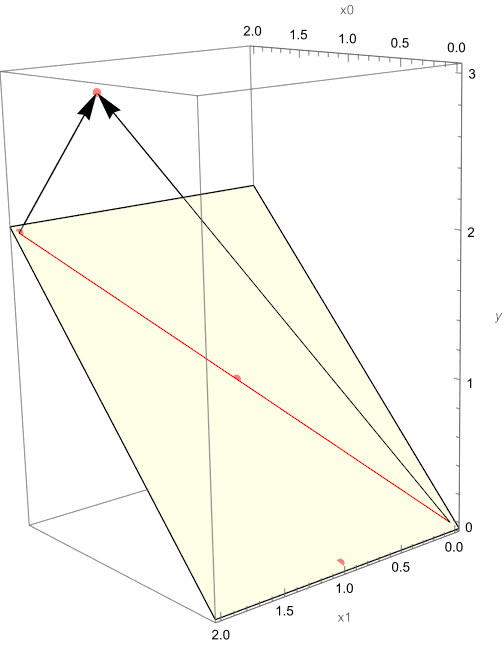
\includegraphics[width=0.30\textwidth]{figures/projection.png}
	\label{fig:projection}
\end{figure}

\end{example}


\end{frame}




\section{Frisch-Waugh-Lovell theorem in matrix algebra}




\begin{frame}{Decomposing the normal equations}
\small
The normal equations in matrix form are $\bm{X}'\bm{X}\bm{b} = \bm{X}'\bm{y}$. If $\bm{X}$ is partitioned into an interesting segment $\bm{X}_2$ and an uninteresting $\bm{X}_1$, normal equations are
\begin{eqnarray}
\begin{bmatrix}
\bm{X}_1'\bm{X}_1 & \bm{X}_1'\bm{X}_2\\
\bm{X}_2'\bm{X}_1 & \bm{X}_2'\bm{X}_2\\
\end{bmatrix}
\begin{bmatrix}
\bm{b}_1\\
\bm{b}_2
\end{bmatrix}=\begin{bmatrix}
\bm{X}_1'\bm{y}\\
\bm{X}_2'\bm{y}
\end{bmatrix}.\nonumber
\end{eqnarray}

The multiplication of the two equations can be done separately
\begin{eqnarray}
\begin{bmatrix}
\bm{X}_1'\bm{X}_1 & \bm{X}_1'\bm{X}_2
\end{bmatrix}
\begin{bmatrix}
\bm{b}_1\\
\bm{b}_2
\end{bmatrix}=\begin{bmatrix}
\bm{X}_1'\bm{y}
\end{bmatrix}\label{first_b1_b2}\\
\begin{bmatrix}
\bm{X}_2'\bm{X}_1 & \bm{X}_2'\bm{X}_2\\
\end{bmatrix}
\begin{bmatrix}
\bm{b}_1\\
\bm{b}_2
\end{bmatrix}=\begin{bmatrix}
\bm{X}_2'\bm{y}
\end{bmatrix}.\label{second_b1_b2}
\end{eqnarray}
How can we find an expression for $\bm{b}_2$ that does not involve $\bm{b}_1$?
\end{frame}


\begin{frame}{Solving for $\bm{b}_2$}
\small
Idea: Solve equation~\eqref{first_b1_b2} for $\bm{b}_1$ in terms of $\bm{b}_2$, then substituting that solution into the equation~\eqref{second_b1_b2}.
\begin{eqnarray}
&&\begin{bmatrix}
\bm{X}_1'\bm{X}_1 & \bm{X}_1'\bm{X}_2
\end{bmatrix}
\begin{bmatrix}
\bm{b}_1\\
\bm{b}_2
\end{bmatrix}=\begin{bmatrix}
\bm{X}_1'\bm{y}
\end{bmatrix}\nonumber\\
&&\bm{X}_1'\bm{X}_1\bm{b}_1+\bm{X}_1'\bm{X}_2\bm{b}_2=\bm{X}_1'\bm{y}\nonumber\\
&&\bm{X}_1'\bm{X}_1\bm{b}_1=\bm{X}_1'\bm{y}-\bm{X}_1'\bm{X}_2\bm{b}_2\nonumber\\
\bm{b}_1&=&(\bm{X}_1'\bm{X}_1)^{-1}\bm{X}_1'\bm{y}-(\bm{X}_1'\bm{X}_1)^{-1}\bm{X}_1'\bm{X}_2\bm{b}_2\nonumber\\
&=&(\bm{X}_1'\bm{X}_1)^{-1}\bm{X}_1'(\bm{y}-\bm{X}_2\bm{b}_2)\nonumber
\end{eqnarray}
Multiplying out equation~\eqref{second_b1_b2} gives
\begin{eqnarray}
&&\begin{bmatrix}
\bm{X}_2'\bm{X}_1 & \bm{X}_2'\bm{X}_2
\end{bmatrix}
\begin{bmatrix}
\bm{b}_1\\
\bm{b}_2
\end{bmatrix}=\begin{bmatrix}
\bm{X}_2'\bm{y}
\end{bmatrix}\nonumber\\
&&\bm{X}_2'\bm{X}_1\bm{b}_1+\bm{X}_2'\bm{X}_2\bm{b}_2=\bm{X}_2'\bm{y}\nonumber
\end{eqnarray}
Plugging in the solution for $\bm{b}_1$ gives
\begin{eqnarray}
&&\bm{X}_2'\bm{X}_1\bigg((\bm{X}_1'\bm{X}_1)^{-1}\bm{X}_1'(\bm{y}-\bm{X}_2\bm{b}_2)\bigg)+\bm{X}_2'\bm{X}_2\bm{b}_2=\bm{X}_2'\bm{y}.
\end{eqnarray}

\end{frame}


\begin{frame}{Solving for $\bm{b}_2$}
\small
\begin{eqnarray}
&&\bm{X}_2'\bm{X}_1(\bm{X}_1'\bm{X}_1)^{-1}\bm{X}_1'(\bm{y}-\bm{X}_2\bm{b}_2)+\bm{X}_2'\bm{X}_2\bm{b}_2=\bm{X}_2'\bm{y}.\nonumber
\end{eqnarray}
The middle part of the first term is $\bm{X}_1(\bm{X}_1'\bm{X}_1)^{-1}\bm{X}_1'$. This is the projection matrix $\bm{P}_{X_1}$ from a regression of $\bm{y}$ on $\bm{X}_1$.
\begin{eqnarray}
&&\bm{X}_2'\bm{P}_{X_1}\bm{y}-\bm{X}_2'\bm{P}_{X_1}\bm{X}_2\bm{b}_2+\bm{X}_2'\bm{X}_2\bm{b}_2=\bm{X}_2'\bm{y}.\nonumber
\end{eqnarray}
We can multiply by an identity matrix $\bm{I}$ without changing anything
\begin{eqnarray}
&&\bm{X}_2'\bm{P}_{X_1}\bm{y}-\bm{X}_2'\bm{P}_{X_1}\bm{X}_2\bm{b}_2+\bm{X}_2'\bm{I}\bm{X}_2\bm{b}_2=\bm{X}_2'\bm{I}\bm{y}.\nonumber\\
&&\bm{X}_2'\bm{I}\bm{y}-\bm{X}_2'\bm{P}_{X_1}\bm{y}=\bm{X}_2'\bm{I}\bm{X}_2\bm{b}_2-\bm{X}_2'\bm{P}_{X_1}\bm{X}_2\bm{b}_2.\nonumber\\
&&\bm{X}_2'(\bm{I}-\bm{P}_{X_1})\bm{y}=\bm{X}_2'(\bm{I}-\bm{P}_{X_1})\bm{X}_2\bm{b}_2.\nonumber\\
\end{eqnarray}
Now $(\bm{I}-\bm{P}_{X_1})$ is the residual maker matrix $\bm{M}_{X_1}$
\begin{eqnarray}
&&\bm{X}_2'\bm{M}_{X_1}\bm{y}=\bm{X}_2'\bm{M}_{X_1}\bm{X}_2\bm{b}_2.\nonumber
\end{eqnarray}
Solving for $\bm{b}_2$ gives
\begin{eqnarray}
\bm{b}_2&=&(\bm{X}_2'\bm{M}_{X_1}\bm{X}_2)^{-1}\bm{X}_2'\bm{M}_{X_1}\bm{y}.\nonumber
\end{eqnarray}

\end{frame}




\begin{frame}{Solving for $\bm{b}_2$}
\small
\begin{eqnarray}
\bm{b}_2&=&(\bm{X}_2'\bm{M}_{X_1}\bm{X}_2)^{-1}\bm{X}_2'\bm{M}_{X_1}\bm{y}.\nonumber
\end{eqnarray}
The residualizer matrix is symmetric and idempotent, such that $\bm{M}_{X_1}=\bm{M}_{X_1}\bm{M}_{X_1}=\bm{M}'_{X_1}\bm{M}_{X_1}$.
\begin{eqnarray}
\bm{b}_2&=&(\bm{X}_2'\bm{M}'_{X_1}\bm{M}_{X_1}\bm{X}_2)^{-1}\bm{X}_2'\bm{M}'_{X_1}\bm{M}_{X_1}\bm{y}\nonumber\\
&=&\bigg((\bm{M}_{X_1}\bm{X}_2)'(\bm{M}_{X_1}\bm{X}_2)\bigg)^{-1}(\bm{M}_{X_1}\bm{X}_2)'(\bm{M}_{X_1}\bm{y})\nonumber\\
&=&(\bm{\tilde{X}}_2'\bm{\tilde{X}}_2)^{-1}\bm{\tilde{X}}_2'\bm{\tilde{y}}.\\
\end{eqnarray}

This is the OLS solution for $\bm{b}_2$, with $\bm{\tilde{X}}_2$ instead of $\bm{X}$ and  $\bm{\tilde{y}}$ instead of $\bm{y}$.
\begin{itemize}
	\item $\bm{\tilde{X}}_2$ are residuals from a regression of $\bm{X}_2$ on $\bm{X}_1$
  \item $\bm{\tilde{y}}$ are residuals from a regression of $\bm{y}$ on $\bm{X}_1$
\end{itemize}
\footnotesize
The solution of the regression coefficients $\bm{b}_2$ in a regression that includes other regressors $\bm{X}_1$ is the same as first regressing all of $\bm{X}_2$ and $\bm{y}$ on $\bm{X}_1$, then regressing the residuals from the $\bm{y}$ regression on the residuals from the $\bm{X}_2$ regression.
\end{frame}



%
%\setlength{\bibsep}{0pt}
%\def\newblock{References} 
%{\footnotesize
%\bibliography{bib}}


\begin{frame}[t,allowframebreaks
]\nocite{*}
\frametitle{References}
\small
\bibliography{bib}
\end{frame}



\end{document}
